% -*- mode:LaTex; mode:visual-line; mode:flyspell; fill-column:75-*-

\chapter{Haptic Design} \label{chapAppendix}
This chapter briefly touches on the field of haptics \ref{hintro} and delves into considerations impacting design \ref{hapticConsiderations}. This leads to a discussion of the requirements \ref{designReq}, initial prototypes \ref{initProto}, and overall challenges which were overcome that led to the development of the final prototype, the vibrotactile array \ref{vibroProto}.

\section{Brief introduction to haptics} \label{hintro}
\textbf{Haptics} are the field of research which concern the sense of touch as it applies to \textit{kinesthetic} and \textit{tactile} sensation. The tactile sense enables humans to perceive object properties through skin contact while the \textit{kinesthetic} or \textit{proprioceptive} sense lets one perceive the positions, movements, and forces on one's own body. 

The skin is lined with an array of sensory receptors which respond to mechanical pressure and distortions such as skin deformation. The \textit{lamellated} or \textit{pacinian corpuscles} (PC) are responsible for sensitivity to vibration and pressure. These rapidly adapting receptors are responsible for vibrotactile perception in glabrous skin. 

Sensitivity to a tactile stimulus grows with the area in contact with the skin and also improves with the stimulus duration until it reaches a point of saturation. When pressure is continuous an effect called \textit{haptic masking} (also known as the \textit{summation effect}) is possible. The overstimulation of the \textit{pacinian corpuscles} causes the brain to ignore these messages with a mechanical filtering system which renders the stimuli to noise in order to focus on other important happenings. If this was not the case, a person could for example feel the pressure exerted by wearing clothing \cite{choi2013vibrotactile}. This phenomena is important to consider when dealing with haptic placement. As mentioned in \ref{tactileModality}, when the vibrotactiles were placed over a larger area haptic masking was avoided and the results closely matched the auditory modality.

\subsection{Haptic Considerations} \label{hapticConsiderations}
The following questions arise based on extensive research done by Choi and Kuchenbecker \cite{choi2013vibrotactile} and are crucial concepts underpinning the creation a meaningful haptic:
\begin{enumerate}
    \item \emph{Can the user feel it?}
Perceptibility of vibrotactile stimuli is strongly dependent on the frequency of vibration. The minimum threshold is observed to be between 150-300Hz and can cover an area smaller than 0.1 micrometer. The absolute thresholds are dependent on factors such as body site, contact area, stimulus duration, stimulus waveform, contact force, skin temperature, presence of other masking stimuli, and age.

    \item \emph{Can the user distinguish between the different vibrotactile cues being displayed?}
This is quantified by the discrimination or \textit{difference threshold} also called the \textit{Just Noticeable Difference} (JND). It is defined as the smallest amount a stimulus intensity much change to produce a noticeable change in sensory experience. The JND is measured as a \textit{Weber fraction}:
${\Delta}$I/I = k or the ratio of difference threshold to the reference level.
Research into experimental psychology has deemed a 20-30\% difference in amplitude or frequency is necessary for robust discrimination between vibrotactile stimuli in practical applications.

    \item \emph{How strong does a certain vibrotactile cue feel to the user?}
\textit{Steven's power law} describes the relationship between the magnitude of a physical stimulus and its perceived intensity or strength. See Figure \ref{fig:StevensPowerLaw}
\begin{figure}[H]
    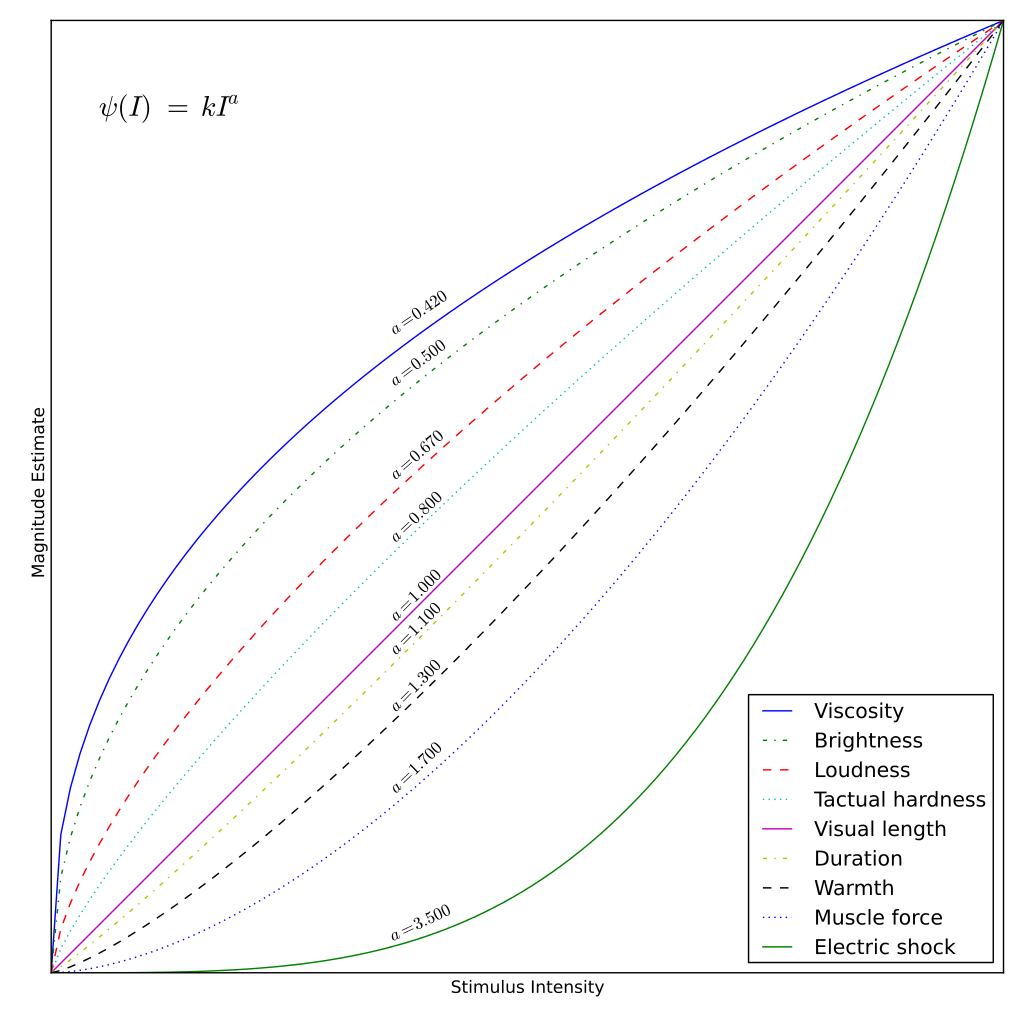
\includegraphics[width=\linewidth,height=\textheight,keepaspectratio]{Steven's_Power_Law}
    \label{fig:StevensPowerLaw}
\end{figure}
When a stimulus intensity \textit{I} is above its absolute threshold, humans perceive its magnitude as \begin{math}\Psi(I)\end{math}(perceptual strength). The exponent (dependent on stimulation freq) determines the growth rate of the perceived magnitude and ranges from 0.35 to 0.86 for vibrotactiles. Perceived intensity is a function of frequency and amplitude of vibration (also affecting perceived pitch).
    \item \emph{How good are users at judging timing of vibrotactile cues?}
Tactile perception is generally considered to have high temporal acuity.
Vibrotactile temporal resolution research cites a human's ability to distinguish successive pulses with a time gap as small as 5 ms (12000 BPM). This resolution is better than vision (25ms) but slightly worse than physiological experiments into the peripheral auditory system which cites a theoretical best case scenario of approximately 2 ms \cite{fishbach2001auditory} \cite{parsons2006neurobiology}. Keep in mind that these are temporal resolutions measured with brain scans and do not necessary translate into the limits of sensorimotor response, which, according to prior research, indicates a more realistic resolution of approximately 50ms.
    \item \emph{Can Vibrotactile cues elicit any other perceptual effects?} Below 3 Hz is considered slow kinesthetic motion. Between 10-70Hz is the sensation of rough motion or fluttering and between 100-300Hz is the sensation of smooth vibration. Subjective quality of a vibrotactile stimulus can be controlled by modifying the envelope of the stimulus amplitude.
\end{enumerate}

\subsection{Vibrotactiles} \label{vibroTT}
The exploration of touch actuation led to the evaluation of available vibrotactiles. The following is a breakdown of available vibrotactiles conducted to inform design perspective.
\begin{enumerate}
    \item Linear electromagetic actuators
    \begin{itemize}
        \item solenoid:
        \begin{itemize}
            \item can leverage resonance, large output for small input
            \item force dependent on position within magnetic field
            \item influenced by device orientation relative to gravity
            \item heats up during use
        \end{itemize}
        \item voice coil:
        \begin{itemize}
            \item linear dynamics yields consistent output, relatively easy to model
            \item \textit{C2 tactor}:
            \begin{itemize}
                \item 7.6mm contactor preloaded against the skin
                \item suspension resonates at 250Hz for maximum perceptibility
            \end{itemize}
            \item \textit{Haptuator}:
            \begin{itemize}
                \item moving magnet design
                \item not meant to touch the skin
                \item optimized to render frequencies above 50Hz
            \end{itemize}
        \end{itemize}
    \end{itemize}
    \item Rotary Electromagnetic Actuators (ERM - eccentric rotating mass)
    \begin{itemize}
        \item simple, reliable, rotate continuously with a constant voltage/current applied
        \item off-center mass affixed to output shaft so that its rotation exerts large radial forces on the body of the motor
        \item couples freq and amplitude of the resulting vibration to the motors rotational speed
        \item small voltage yields weaker vibrations
        \item intrinsic spin-up time could cause delay at the start of the cue
        \item internal static friction can prevent motor from rotating when the applied voltage is very small
    \end{itemize}
    \item Nonelectromagnetic Actuators - Piezoelectric effect
    \begin{itemize}
        \item respond to inputs very quickly and can output arbitrary waveforms
        \item typically require input on the order of 100V
        \item high stiffness of skin creates a need for relatively heavy vibrotactile actuator
        \item most don't have power to move the skin without pushing off a cumbersome mechanical ground
    \end{itemize}
    \item EAP (electroactive polymer) actuators
    \begin{itemize}
        \item uses elastomers rather than ceramics
        \item can achieve larger deformations for lower drive voltages
    \end{itemize}
    \item SMA (shape memory allow) actuators
    \begin{itemize}
        \item remembers original shape
        \item mechanical properties altered in response to temp changes
        \item slow response time, large hystoresis, high energy consumption
    \end{itemize}
    \item Pneumatic systems
    \begin{itemize}
        \item compact, light
        \item require high-pressure air source
        \item struggle to output high-frequency signals
    \end{itemize}
    \item Forced impact
    \begin{itemize}
        \item TacHammer - new technology, specs unknown, hard to acquire
    \end{itemize}
\end{enumerate}

\subsubsection{Vibrotactile Constraints}
\begin{enumerate}
    \item Create consistent mechanical coupling between actuator vibrations and users skin
    \item Slight changes to such a system drastically affect a users ability to feel and comprehend the rendered signals.
    \item For fixed actuator size/activation level, magnitude of created vibrations is inversely proportional to the mass of the object.
    \item High bandwidth accelerometer can be used to measure vibration output performance \cite{ignoto2017development}.
    \item When the application involves a large object, a wearable device, and/or multiple stimulation sites, the optimal vibrotactile rendering paradigm is to vibrate one or more small zones. 
    \begin{itemize}
    \item In a tactile display application the localization accuracy of 250-Hz vibrotactile stimuli around the waist was 74\% with 12 equidistant tactile actuators (tactors), 92\% with eight tactors, and 97\% with six tactors \cite{choi2013vibrotactile}.
    \end{itemize}
\end{enumerate}

\section{Design requirements} \label{designReq}

The initial requirement set forth by Professor Neely in the Haptic Enviro-Sensing Metronome (HESM) design draft is centered around an analogue wave that could squeeze and release. As the analogue wave approaches its crest it provides insight forecasting the approaching \textit{crusis}, allowing the user to prepare for and rebound from the "click-moment" with rich entrainment. 

This observation is in direct parallel to external vibrotactile metronome research as discussed in \ref{vibrotactileMetronome}. The constraint was such that the pulses should feel continuous and not discrete in order to capture the essence of pendulum motion.

As the intention is to encourage entrainment of the human body to external forces, the frequencies
required are quite low, based on the tempi of slow walking to running gaits
(40 bpm/.67 Hz to 180 bpm/3 Hz).

\section{Initial Prototypes} \label{initProto}
In order to capture the sensation defined in the design requirements, a series of prototypes were rapidly developed.

\subsection{Solenoid bracelet}
Initial introspection towards capturing the squeeze and release sensation led to the rapid prototyping of a simple solenoid bracelet. 
\subsubsection{Parts List}
\begin{enumerate}
    \item Adafruit Pro Trinket 5V 16MHz
    \item N-channel MOSFET
    \item 1N4004 diode
    \item mini push-pull solenoid
\end{enumerate}
\subsubsection{Assembly}
The design was inspired and assembled per \textit{Adafruit} specification \cite{Solenoid}. 
The base of an N-channel MOSFET was connected through a 1K resistor to a digital I/O pin on the trinket per Figure \ref{SolenoidSchematic}. The collector was connected through the solenoid and diode in parallel to Vcc running at 5V.
\begin{figure}[H]
    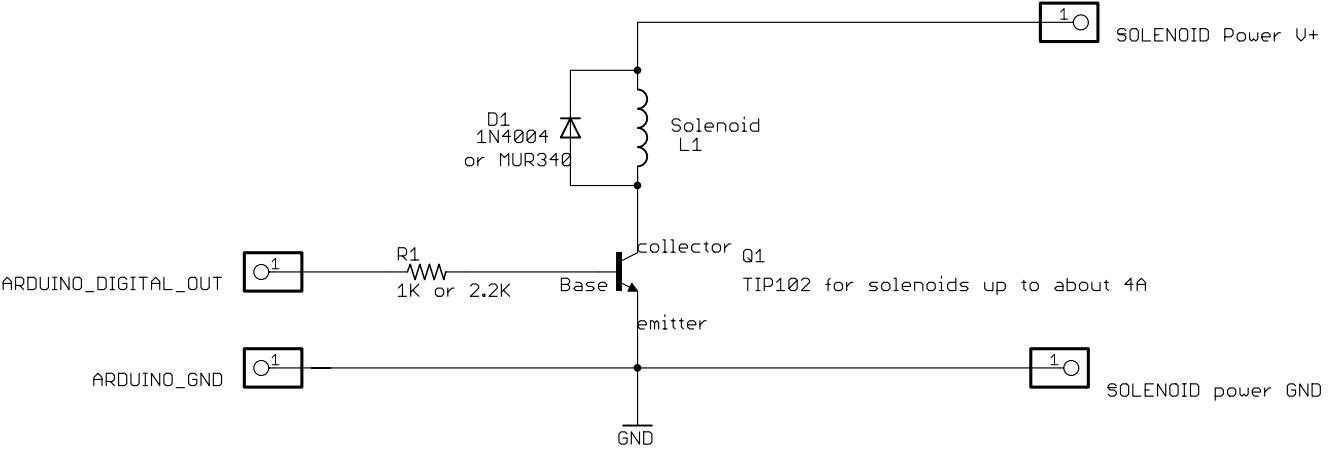
\includegraphics[width=\linewidth,height=\textheight,keepaspectratio]{Solenoid_Schematic}
    \caption{Solenoid Schematic}
    \label{SolenoidSchematic}
\end{figure}
\subsubsection{Method}
    As a voltage is applied the slug in the middle of the solenoid is pulled into the center of the coil. The actuation pulls a taught wristband attached to the chasis of the solenoid and as the voltage drops the solenoid retracts releasing tension in the wristband, shown in Figure \ref{SolenoidProto}.
    
    \begin{wrapfigure}{R}{.5\textwidth}
        \centering
        \caption{Solenoid Wristband Prototype}
        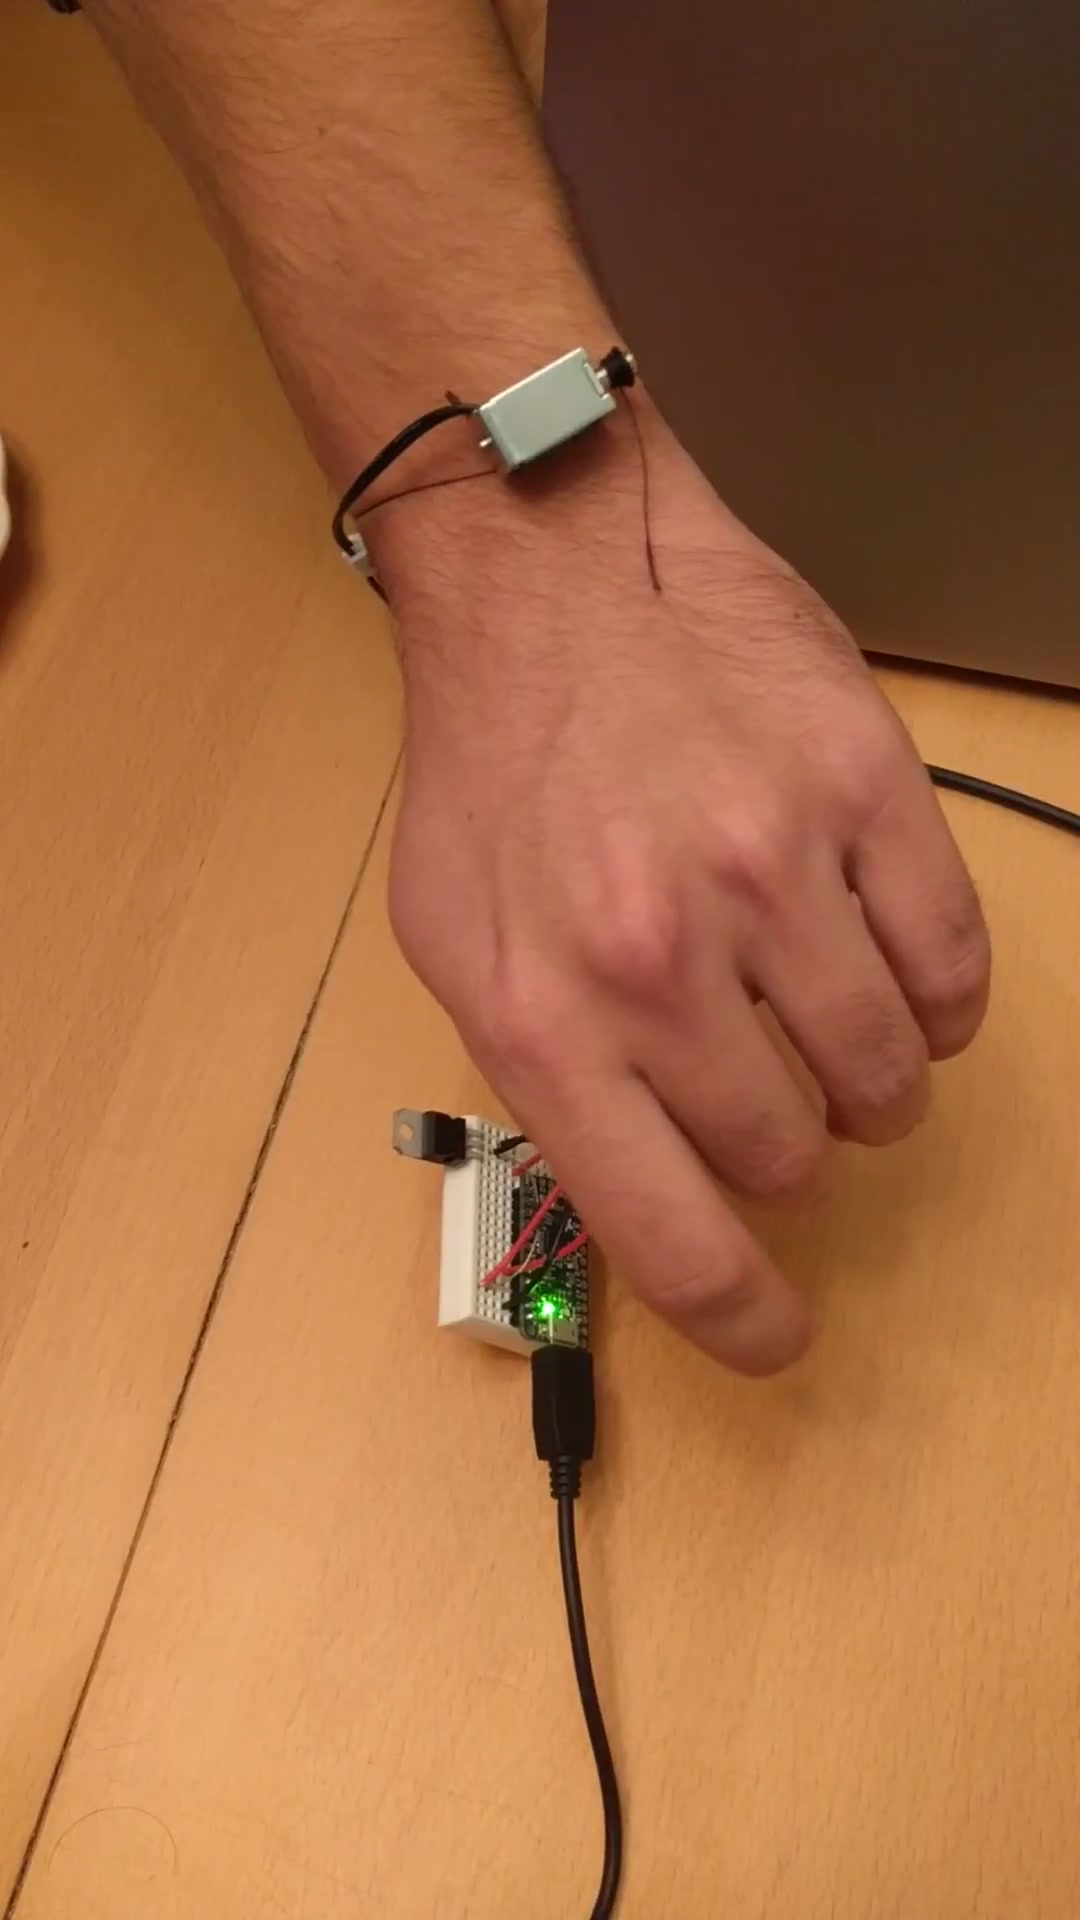
\includegraphics[width=.5\linewidth,height=.5\textheight,keepaspectratio]
        {SolenoidProto}
        \label{SolenoidProto}
    \end{wrapfigure}
    
    This was controlled in the \textit{Arduino IDE} through a simple PMW signal with increasing duty cycle which output through the digital I/O. The delay was hard coded proportional to the desired BPM.

\subsubsection{Outcome}

Due to the linear relationship between current draw and pull force, the solenoid required high current and significant voltage thus isolation from the microcontroller was ideal. The necessary rigidity of the band was a cause of discomfort and the lack of positioning options was a detriment to musicians who relied on availability of their hand. Additionally, heat dissipation was at times unsafe and unbearable since the chasis was in direct contact with the skin. Though it captured the tension and release sensation well, there seemed to be a lack of clarity with regards to communication of whether each push pull iteration was a beat length or if a single contraction was the downbeat (i.e. eighth note pulse rather than quarter note). Coupled with the bulky nature of the solenoid chasis, high power requirements and excessive heat dissipation, the solenoid prototype was quickly abandoned.
\subsection{Single vibrotactile}

The subsequent prototype iteration was the first involving a vibrotactile motor. Since the goal was to run everything off of a single board, the voltage constraint was limited to the 5V maximum per \textit{Adafruit Pro Trinket} spec. An ERM motor was chosen for its working voltage range of 2-5V and minimal coin cell form factor (10mm diameter). Like the solenoid, higher applied voltage yielded more current draw but stronger vibration. At 5V, a single motor draws 100mA. The specification was 1100 at 5V which roughly translates to 183Hz. Though not quite at the ideal 250Hz range optimal for skin sensitivity, this was deemed close enough.

To realize the spectrum of capability for vibrotactile sensation (beyond pulse width modulation of the signal) a haptic motor controller with a pre-installed library of effects was acquired. 

The goal of this design was to test the ERM sensation on a portable wearable. The MCU was altered from the Pro Trinket to the Flora which ran at 3.3V and had less digital I/O pins, but supported external connectivity and took up less surface area.

\subsubsection{Parts List}
\begin{enumerate}
    \item Vibrating mini motor disc
    \item Adafruit DRV2605L Haptic Motor Controller
    \item Flora Wearable Bluefruit LE Module
    \item Flora Wearable electronic platform
    \item LiPo Battery - 3.7v 1100mAh
\end{enumerate}
\subsubsection{Assembly}
    First, the ERM leads were soldered to the DRV2605 haptic motor controller and connected via I2C protocol to the complimentary pins on the Flora (SCL,SDA).
    To experiment with triggering the vibrotactile wirelesssly, the bluetooth low energy (BLE) module was added and the send and receive (Tx/Rx) pins were connected as referenced in Figure \ref{fig:Proto2}. The battery was connected via the built-in terminal clip and last the entire prototype was fitted into the space of a sports wristband with the vibrotactile on the inside touching the skin.

    \begin{figure}[H]
        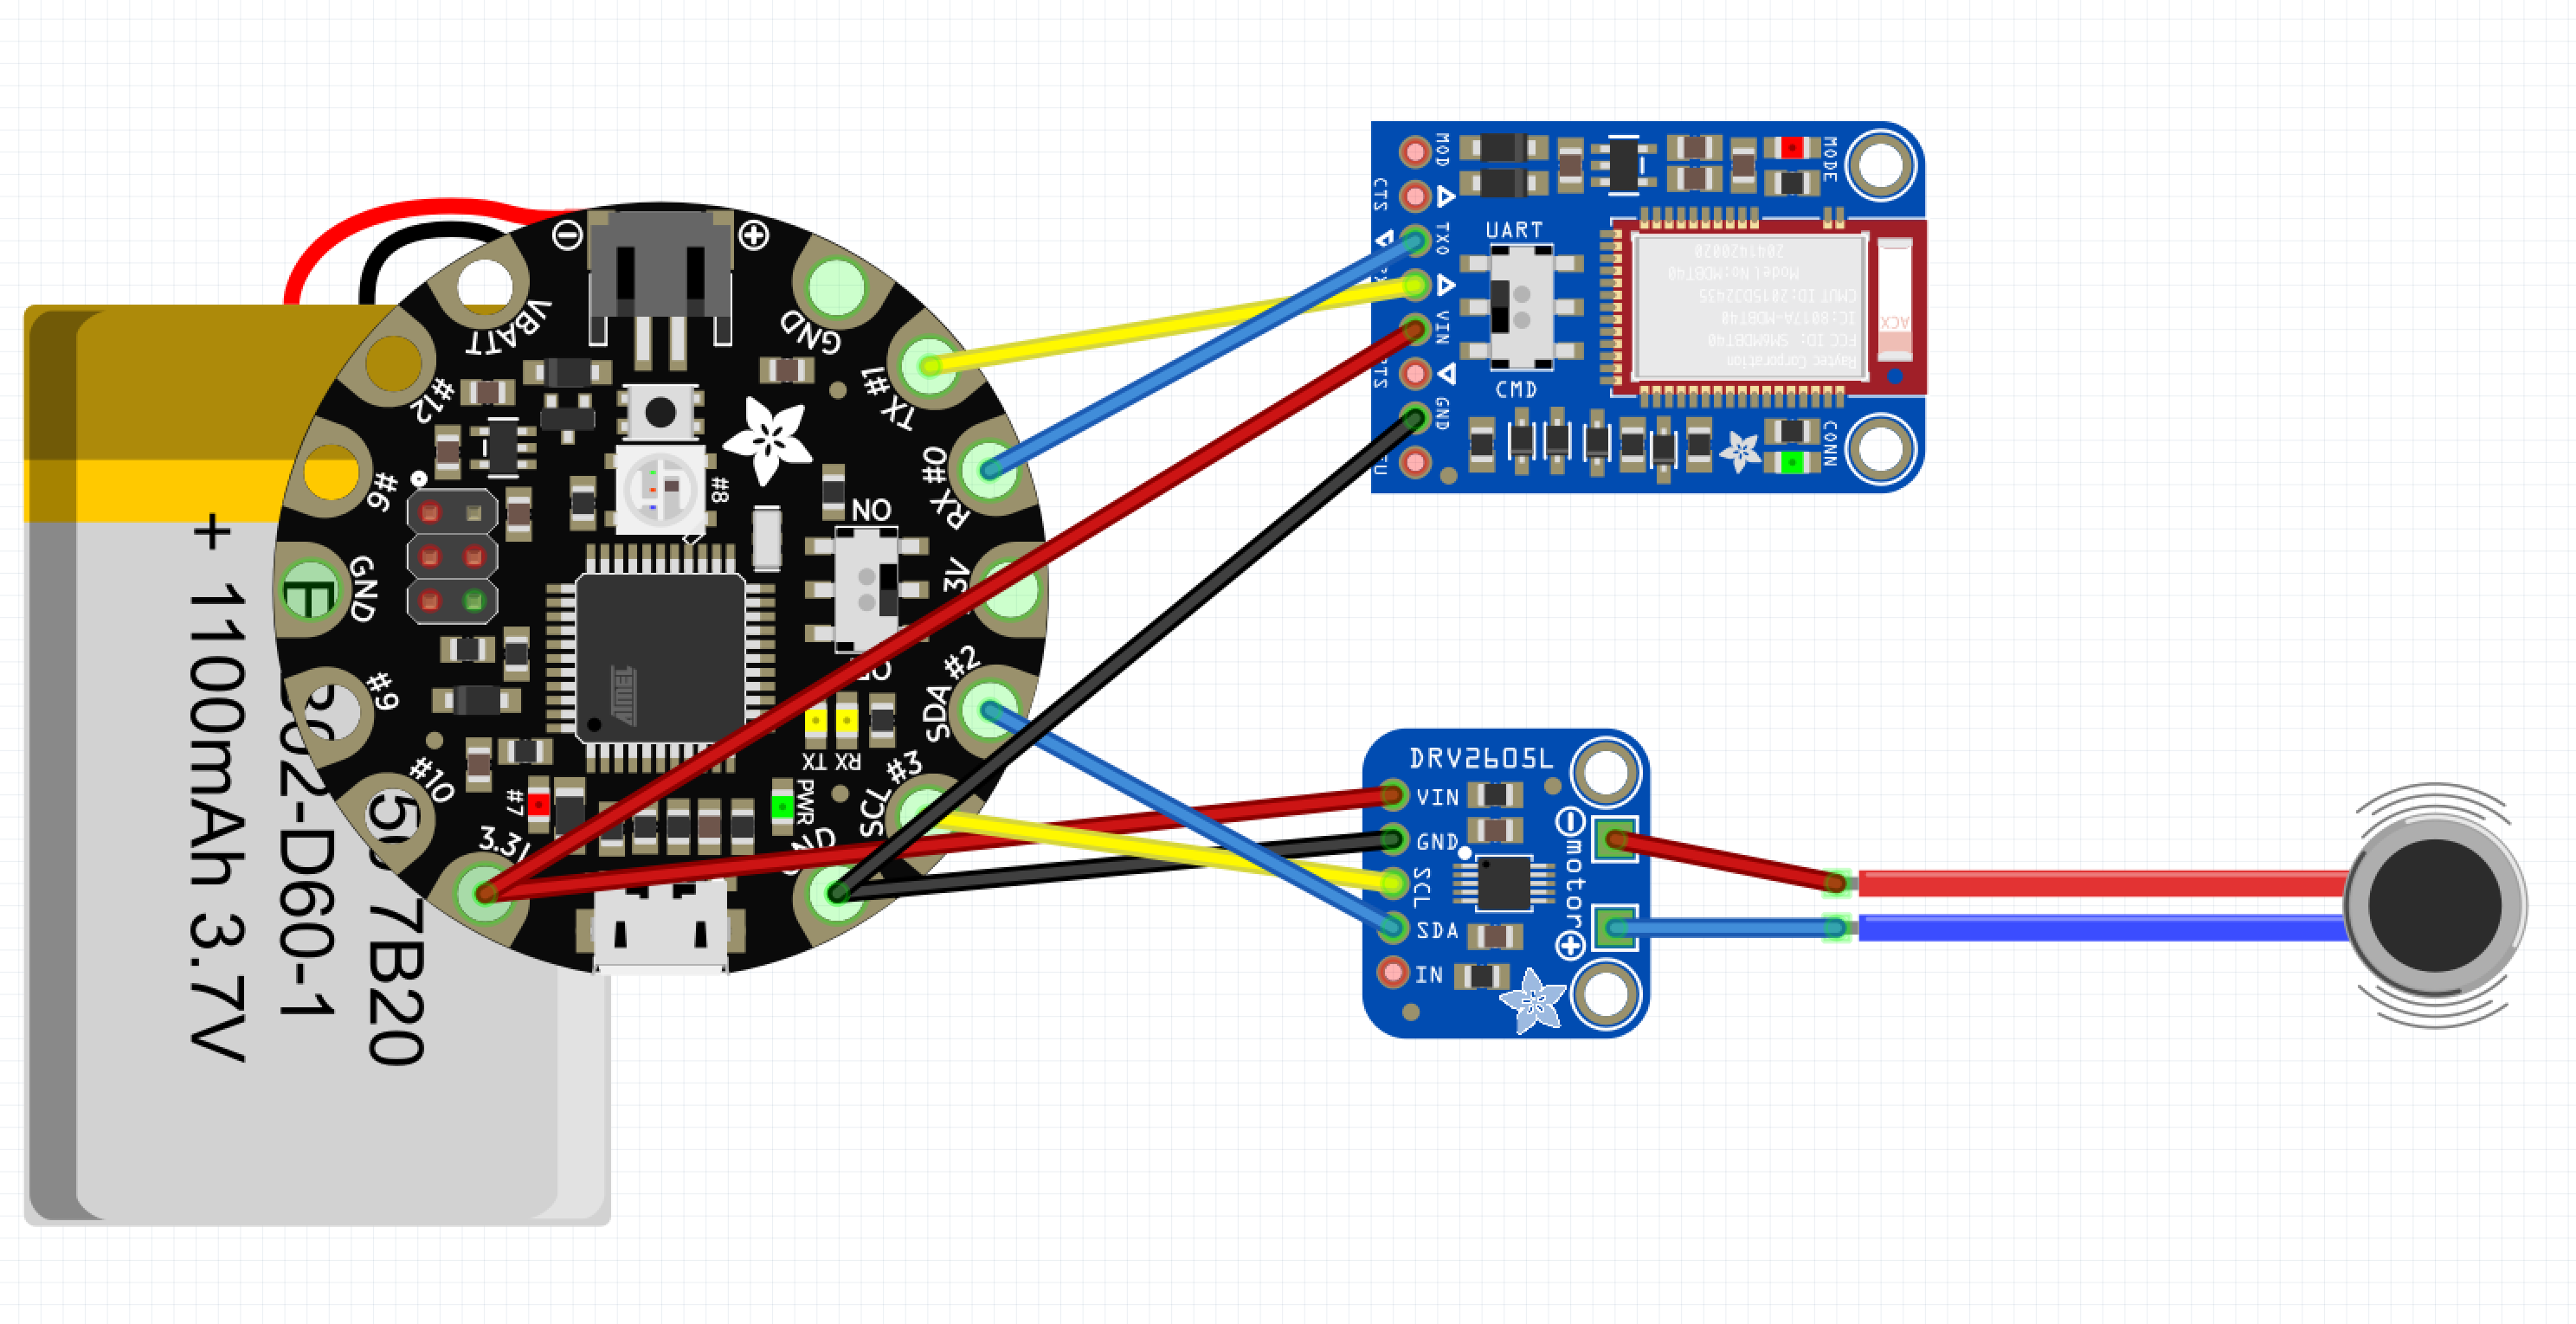
\includegraphics[width=\linewidth,height=\textheight,keepaspectratio]{Proto2_bb}
        \caption{Prototype 2 - Single vibrotactile, wireless connectivity}
        \label{fig:Proto2}
    \end{figure}

\subsubsection{Method}
    Once the hardware was setup, the haptic library was iterated through for selection of the most influential effect. The optimal sensation chosen was a queue of two chained effects according to the \underline{DRV2605 datasheet}\cite{Adafruit}:
    \begin{itemize}
        \item 83 - Transition Ramp Up Long Smooth 2 - 0 to 100\%
        \item 71 - Transition Ramp Down Long Smooth 2 - 100\% to 0
    \end{itemize}

    Within the Arduino IDE the Bluefruit library and dependencies were imported and the bluetooth low energy connection configured via UART. On the client side, the connectivity was validated via the publicly available Bluefruit application on an external Android device. The app would send integer values representing the desired BPM to the connected haptic wearable. The code was written such that upon setup and BT pairing, the main loop was polling for packets. Once received in the buffer, the new bpm value was parsed into a period value in milliseconds via equation \ref{eq:period}

    \begin{equation}
        \label{eq:period}
        period = \frac{60,000}{bpm}
    \end{equation}

    Since the highest operational bpm specified was 180, the shortest period would be an interval of 333.33 ms. This value divided in half gave the maximum allowed ramp up time for the motor, approximately 150ms. The new period value was fed into a state machine which set the on and off state of the motor based on a timer from half the calculated period as well as the 150ms off state.

    \subsubsection{Outcome}
    The singular ERM prototype granted key insight into the capability of a vibrotactile to create the desired awareness and fill the interstitial space; though it was found to be lacking the ability to fully command the wearer's attention. This was primarily due to the fact that it was driven by a 3.3V board which inhibited the vibrational strength. The next iteration needed to operate at higher voltage to get a stronger vibration. It was also deemed necessary to increase the number of vibrotactiles to work in an array format in complete synchronicity to explicitly communicate the necessary ramp down and up sensation. 
    
    Though the haptic motor controller was a critical evaluation tool for selecting the vibration effect, it was crucial for the final prototype to be able to turn on the motors at full voltage as quick as possible in order to minimize ramp up time. Chaining the motors would also optimize ramp up time in allowing a motor the time to fully spin back down while the adjacent was spinning up.

    Furthermore, the \textit{delay()} function added in the BLE section of code was causing the haptic to drift slightly in tempo beyond five minutes of runtime due to the programmatic halting and resumption of dependent timers. The next prototype would have to move away from the delay function which halted program execution.

\section{Vibrotactile Haptic Array} \label{vibroProto}
The final prototype was an array of four vibrotactiles. Several hardware advancements were implemented in order to solve design challenges. The overall process is detailed below.
\subsection{Hardware}
The main board was reverted back to that used in the solenoid prototype, the 5V 16MHz \textit{Adafruit Pro Trinket}, in order to provide maximum possible voltage to the motors. This board did not have built in serial communication so an FTDI to USB cable was necessary in order to communicate with the device. Bluetooth connectivity was abandoned to concentrate focus on minimized latency. 
\subsubsection{Parts List}
\begin{table}[H]
    \centering
    \resizebox{\columnwidth}{!}{%
    \begin{tabular}{lll}
    Part Type & Properties & Quantity \\ \hline
    Electrolytic Capacitor & capacitance 68µF; package 0405 {[}SMD, electrolytic{]}; voltage 16V & 1 \\
    Electrolytic Capacitor & capacitance 10µF; package 200 mil {[}THT, electrolytic{]}; voltage 25V & 4 \\
    Ceramic Capacitor & capacitance 100nF; package 100 mil {[}THT, multilayer{]}; voltage 6.3V & 1 \\
    Diode & package diode-1n4001; variant pth & 4 \\
    Vibration Motor & vibration motor 11000 RPM 5VDC & 4 \\
    Adafruit Pro Trinket 5V 16MHz & variant variant 1; part \# Adafruit \#2000 & 1 \\
    2N7000 FET N-Channel & package TO92; type n-channel; part \# 2N7000 & 4 \\
    220Ω Resistor & tolerance ±5\%; package 0805 {[}SMD{]}; resistance 220Ω & 5 \\
    10kΩ Resistor & tolerance ±5\%; package 0603 {[}SMD{]}; resistance 10kΩ & 1 \\
    FTDI to USB & Adafruit FTDI Serial TTL­232 USB Cable {[}ADA70{]} & 1 \\
    Shrink wrap & Heat Shrink Pack & 1
    \end{tabular}%
    }
    \caption{Vibrotactile Haptic Array Parts List}
    \label{Vibrotactile Haptic Array Parts List}
\end{table}

\subsubsection{Assembly}
Since each digital I/O of the Trinket could only source 20mA, four N-channel 2N7000 transistors were chosen to act as switches and current isolators for controlling power to the motors. These are labelled (N) in Figure \ref{FinalProto}

Each motor was connected from the power source (5V Vcc), to the drain of the transistor. When the transistor received a signal past its bias voltage of 0.8V it was switched on. This allowed the drain-source channel to be opened and an onrush of current to flow from Vcc to the motors and through to ground. 

A 1N4001 diode was placed in parallel with the motor from the 5V Vcc node to the drain of the N-channel 2N7000 to protect the transistor by shorting out the onrush of back current emitted from the motor during immediate shutoff. Principally, the motor will act as an inductor; a sudden change in current creates an equivalent voltage to keep that current flowing short term. This could fry the transistor if the diode was not in place to short out this negative voltage spike as shown in \ref{fig:MotorRinging} 
\begin{figure}[H]
    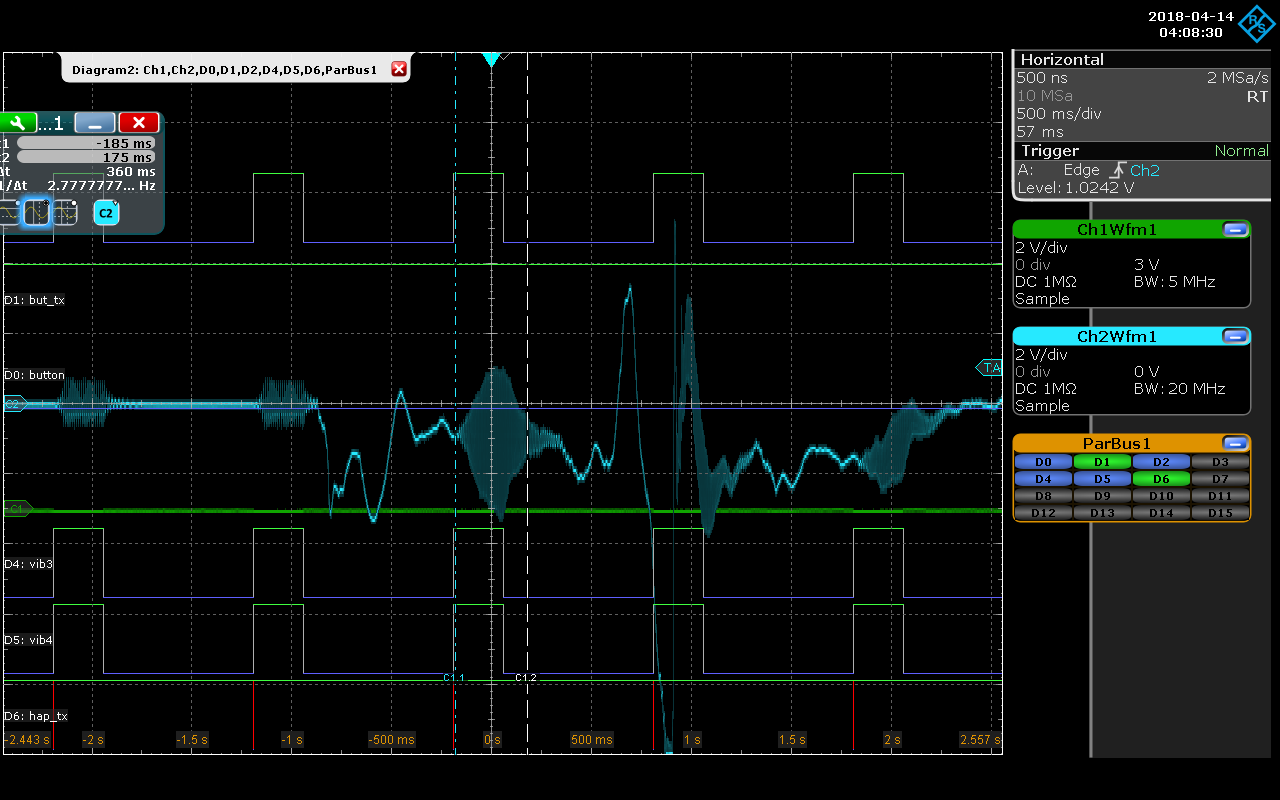
\includegraphics[width=\linewidth,height=\textheight,keepaspectratio]
    {ringing}
    \caption{Motor ringing after abrupt shutoff}
    \label{fig:MotorRinging}
\end{figure}

The digital pins 5,6,9,10 (denoted with yellow and grey wires in Figure \ref{fig:FinalProto}) output a pulse-width modulated signal to be used as triggers, or control switches, for the transistors. In order to limit the current that the digital output must source and to protect the transistor gate, a 220 Ohm resistor was connected across the digital I/O pin and the gate of the 2N7000 for each pin.

\begin{figure}[H]
    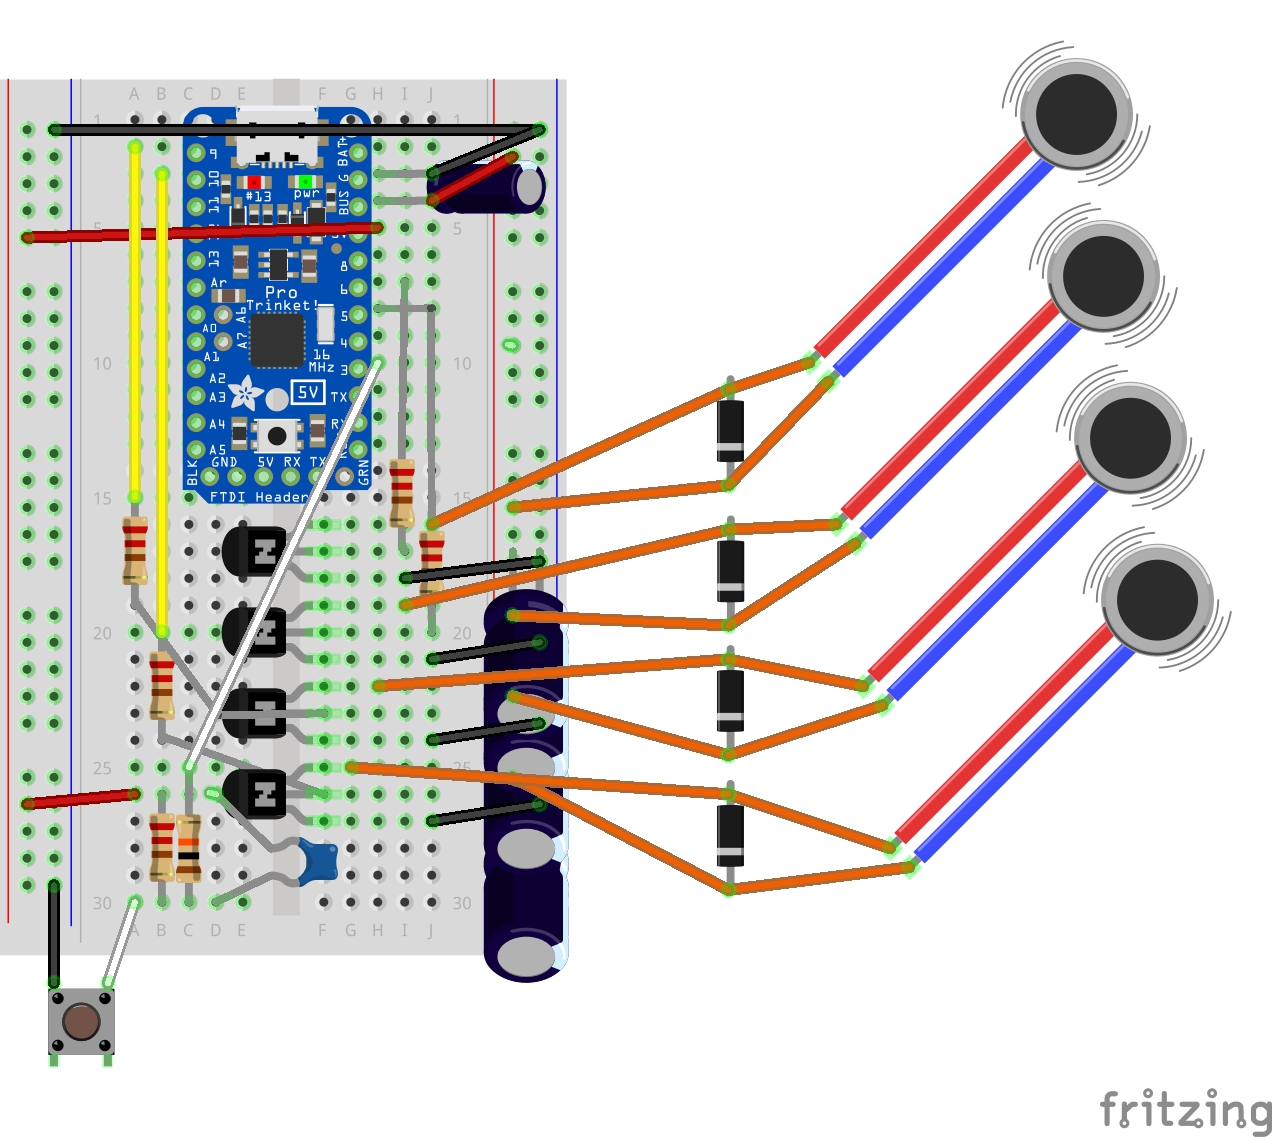
\includegraphics[width=\linewidth,height=\textheight,keepaspectratio]
    {FinalProto_bb}
    \caption{Final prototype wiring mockup}
    \label{fig:FinalProto}
\end{figure}

The voltage across the rails (Vcc and ground) was viewed on a Rohde \& Schwarz RTO 2004 oscilloscope. The analyzed waveform showed some unfavorable dips primarily when all motors were running due to the high current draw from the ERMs in addition to some ringing (overshoot), seen in Fig \ref{fig:precaps}.
\begin{figure}[H]
    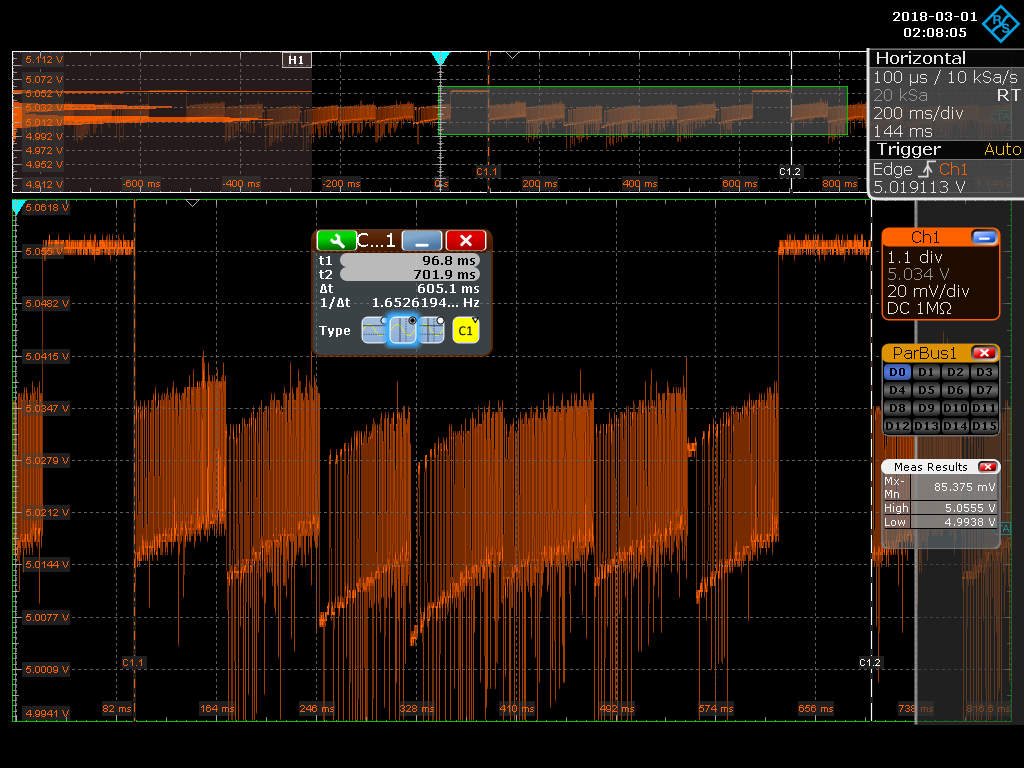
\includegraphics[width=\linewidth,height=\textheight,keepaspectratio]
    {pre-cap}
    \caption{V drop across Vcc and HF ringing: Pre-cap}
    \label{fig:precaps}
\end{figure}
\subsection{Improvements}
Capacitors were added to act as buffers from the power source to the motors, in doing so they helped provide immediate current to the motors when the PWM input signal engaged the transistor and the motor would go from an off state to an immediate on state drawing high amounts of current. Large electrolytic capacitors are known for their ability to supply high currents for a few milliseconds, more so than a battery or in the haptic wearables case, USB power. These were added across Vcc and ground nearest to the Trinket as well as across each of the node rails nearest to the motors. The change in output shape can be analyzed in Fig \ref{fig:postcaps}.

\begin{figure}[H]
    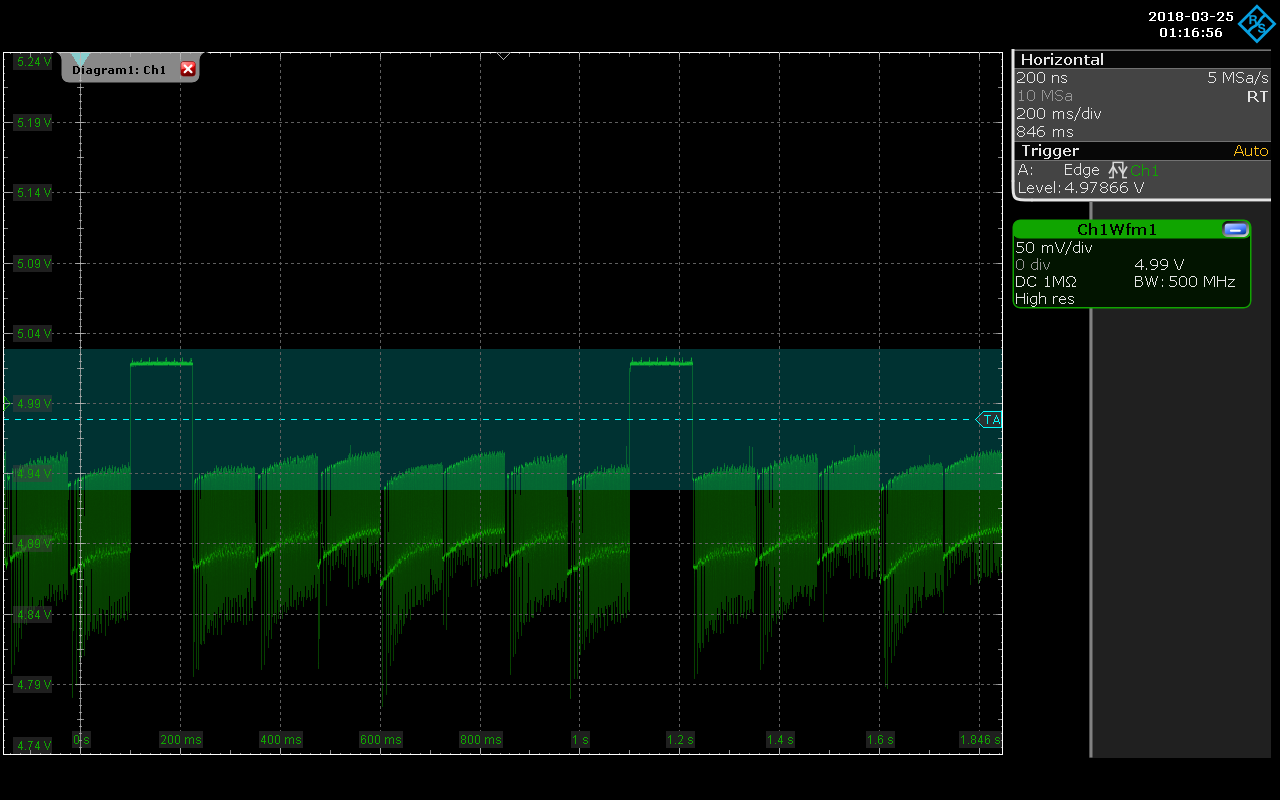
\includegraphics[width=\linewidth,height=\textheight,keepaspectratio]
    {post-cap}
    \caption{V drop across Vcc: Post-cap}
    \label{fig:postcaps}
\end{figure}

As an additional manual tap tempo option for the user to experiment with, a push-button was added and connected to the only interrupt capable pin on the Trinket, PIN 3. An RC combination was chosen to act as a low-pass filter to protect against debounce scenarios.

\begin{figure}[H]
    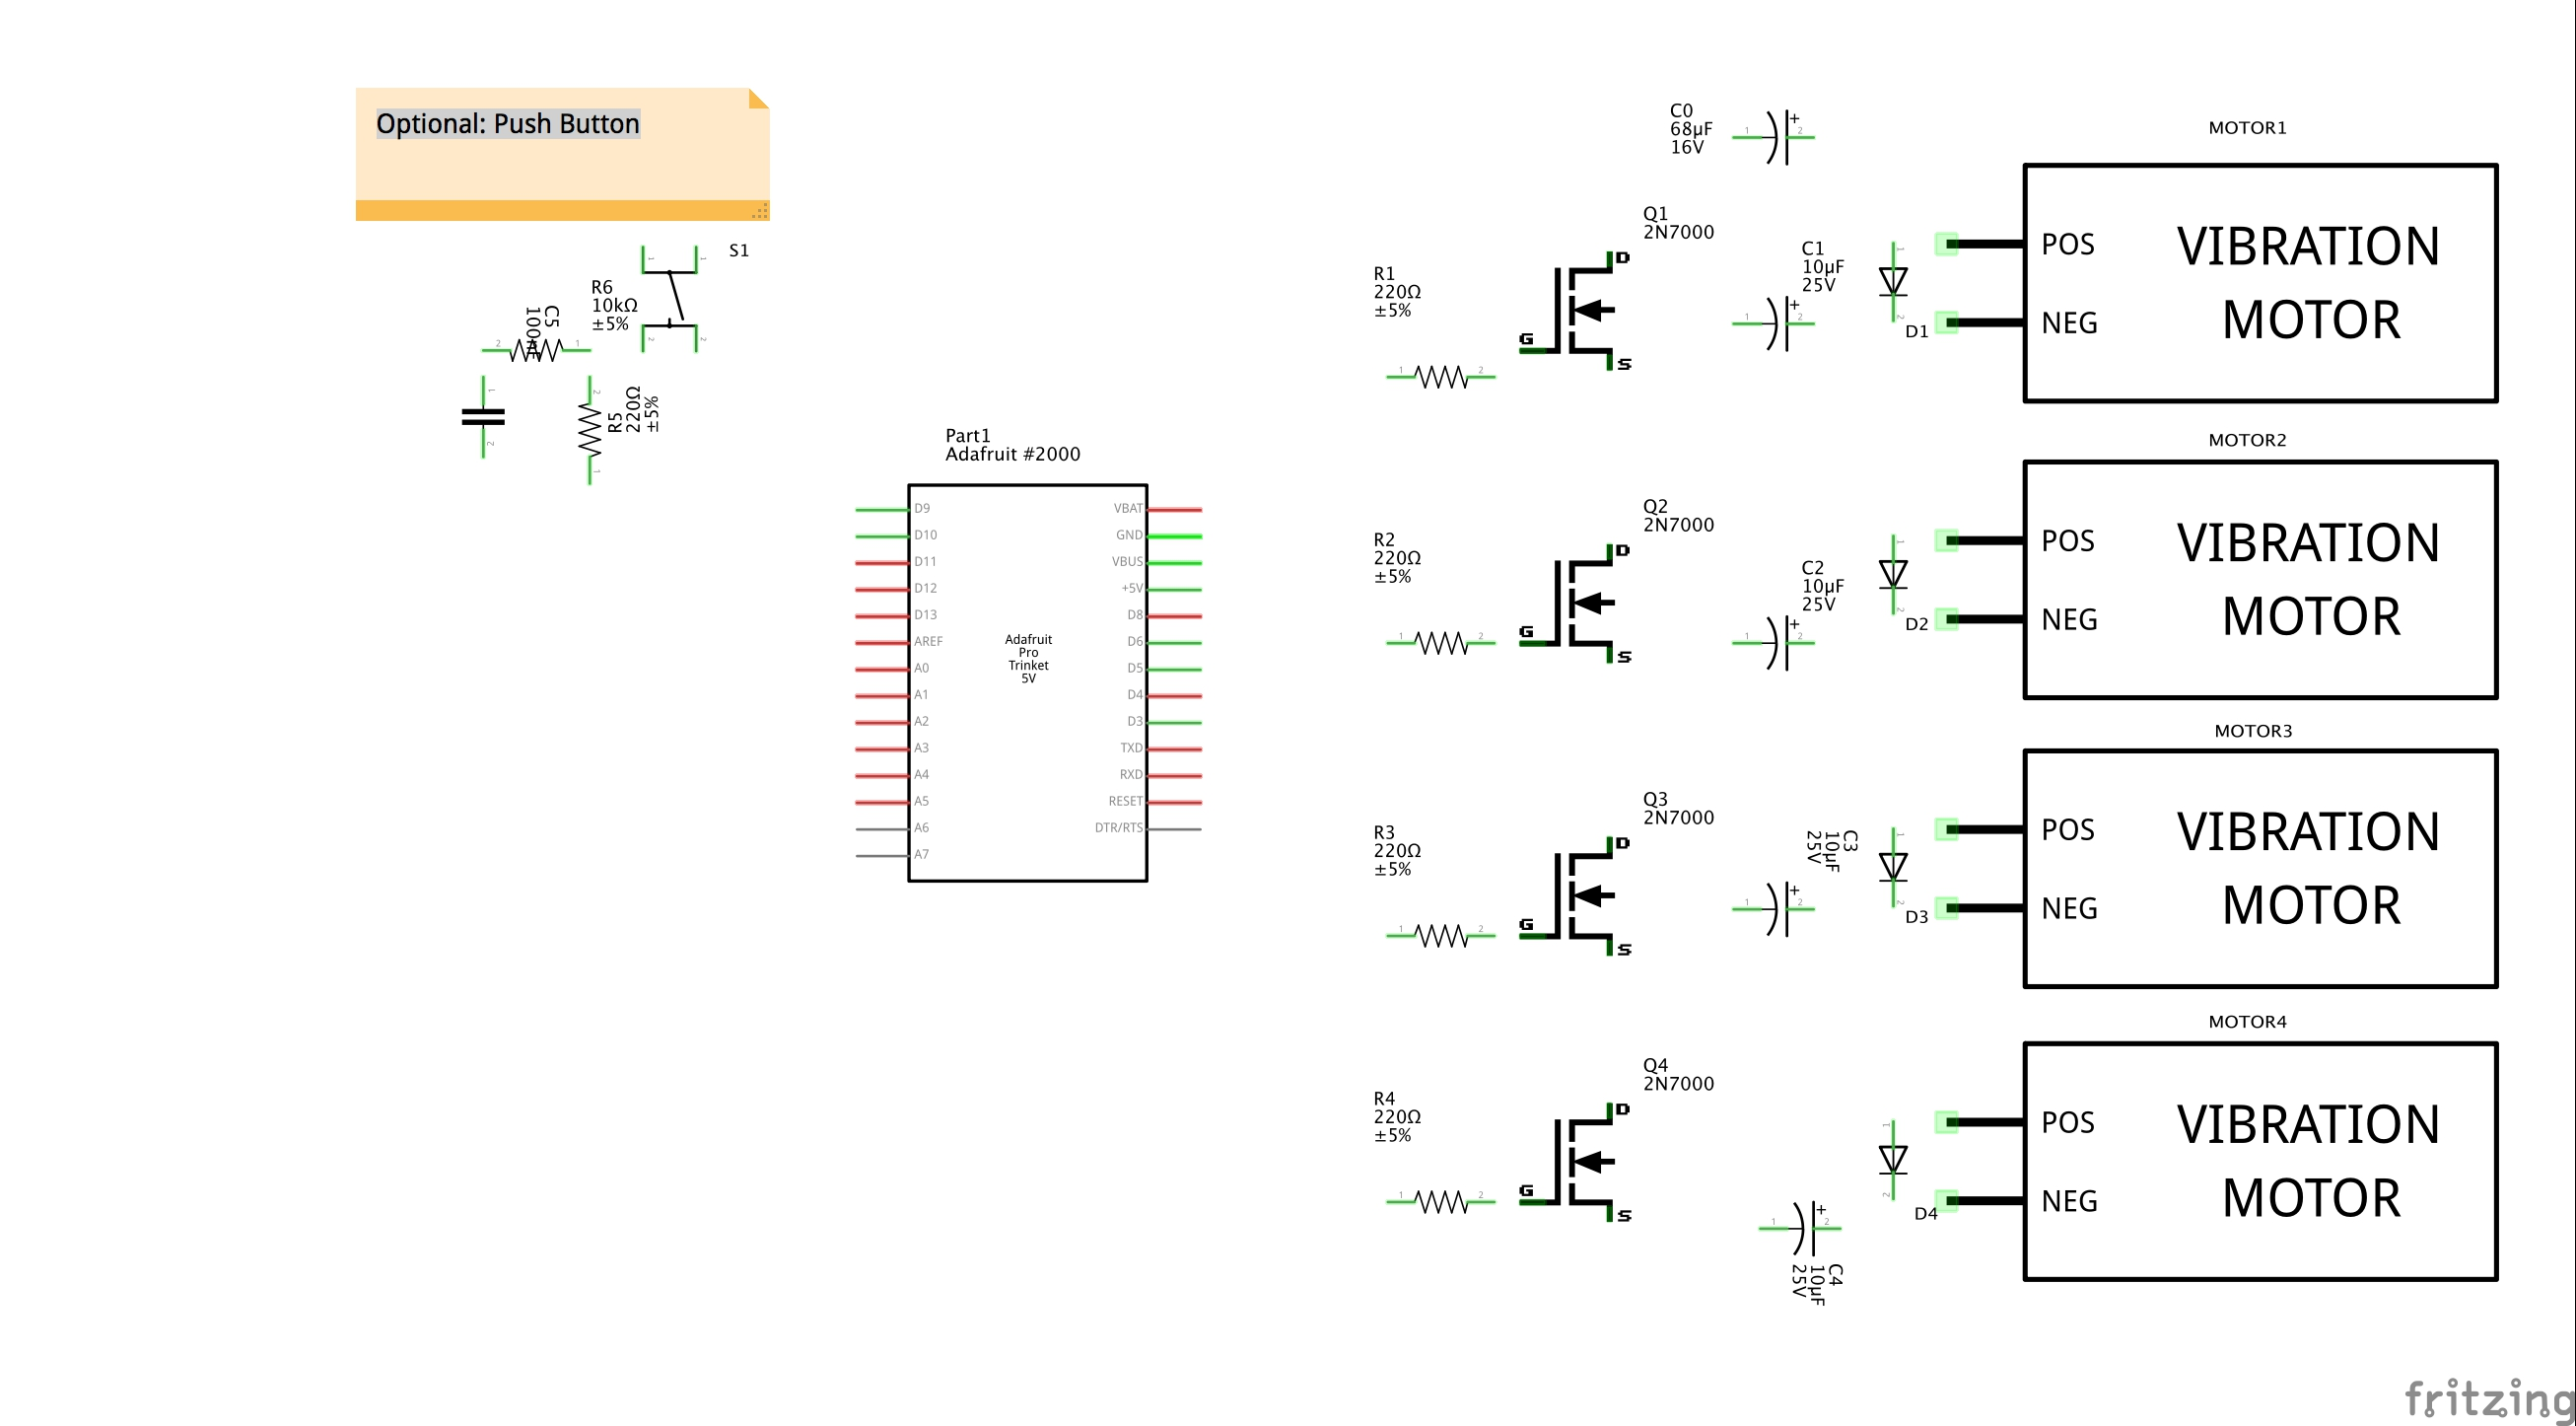
\includegraphics[width=\textwidth,height=\textheight,keepaspectratio]
    {FinalProto_schem}
    \caption{Final prototype abstracted schematic}
    \label{fig:FinalProtoSchem}
\end{figure}

\subsubsection{Motor Characterization}
In order to determine an accurate baseline for motor ramp up, a singular motor was firmly attached to a piezoelectric transducer. The remaining motors were connected to the digital bus of the scope for timing analysis. 
\begin{figure}[H]
    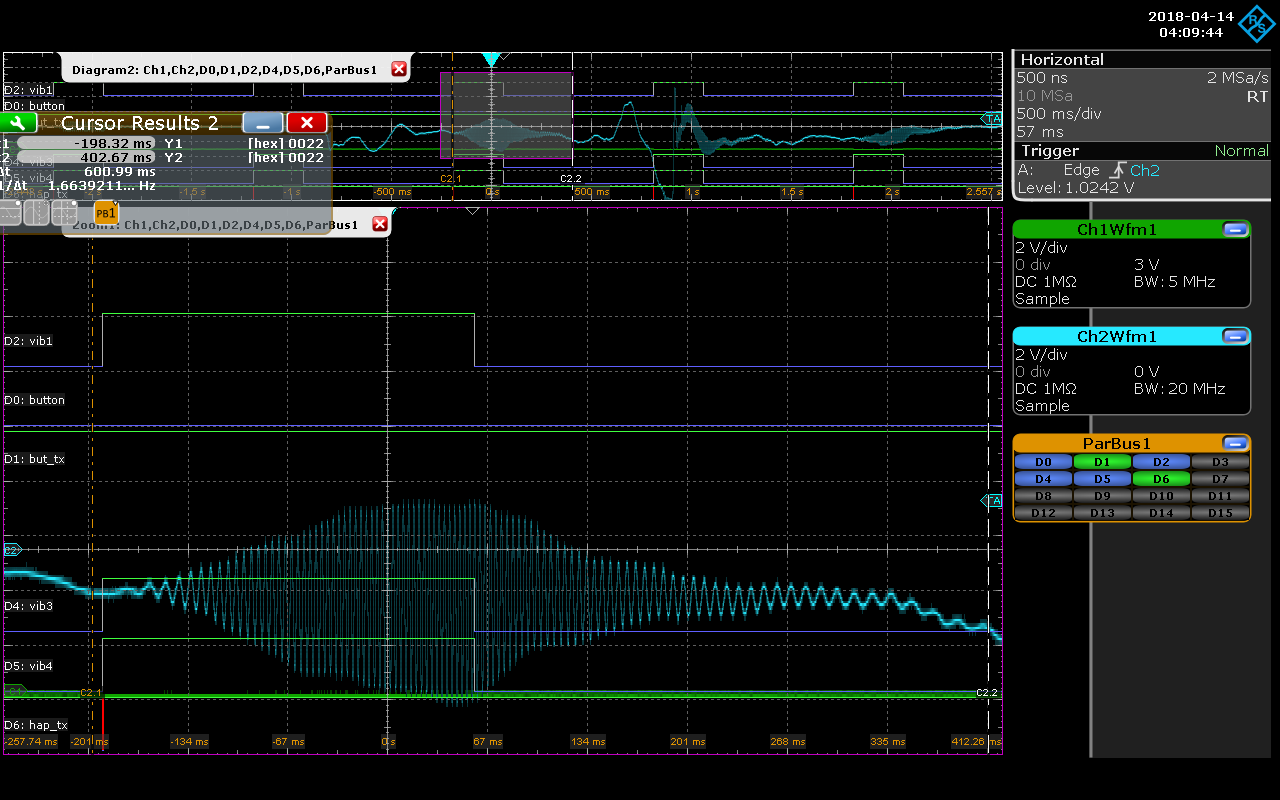
\includegraphics[width=\textwidth,height=\textheight,keepaspectratio]
    {motorramp}
    \caption{Motor ramp up time}
    \label{fig:MotorRampUp}
\end{figure}

As seen in Fig \ref{fig:MotorRampUp}, the motors reach full amplitude over approximately 67ms before the signal goes low and starts to decay. The AC shape of the waveform is due to the nature of the ERM. The rotating mass translates left and right movement into a voltage oscillating in amplitude. Multiple ramp up times were averaged using this method such that the time before perceptibility was determined to be about a quarter of the ramp up time (approximately $50ms$), in agreement with \ref{HD}. This is clearly shown in Fig \ref{fig:MotorRampUp2} below.
\begin{figure}[H]
    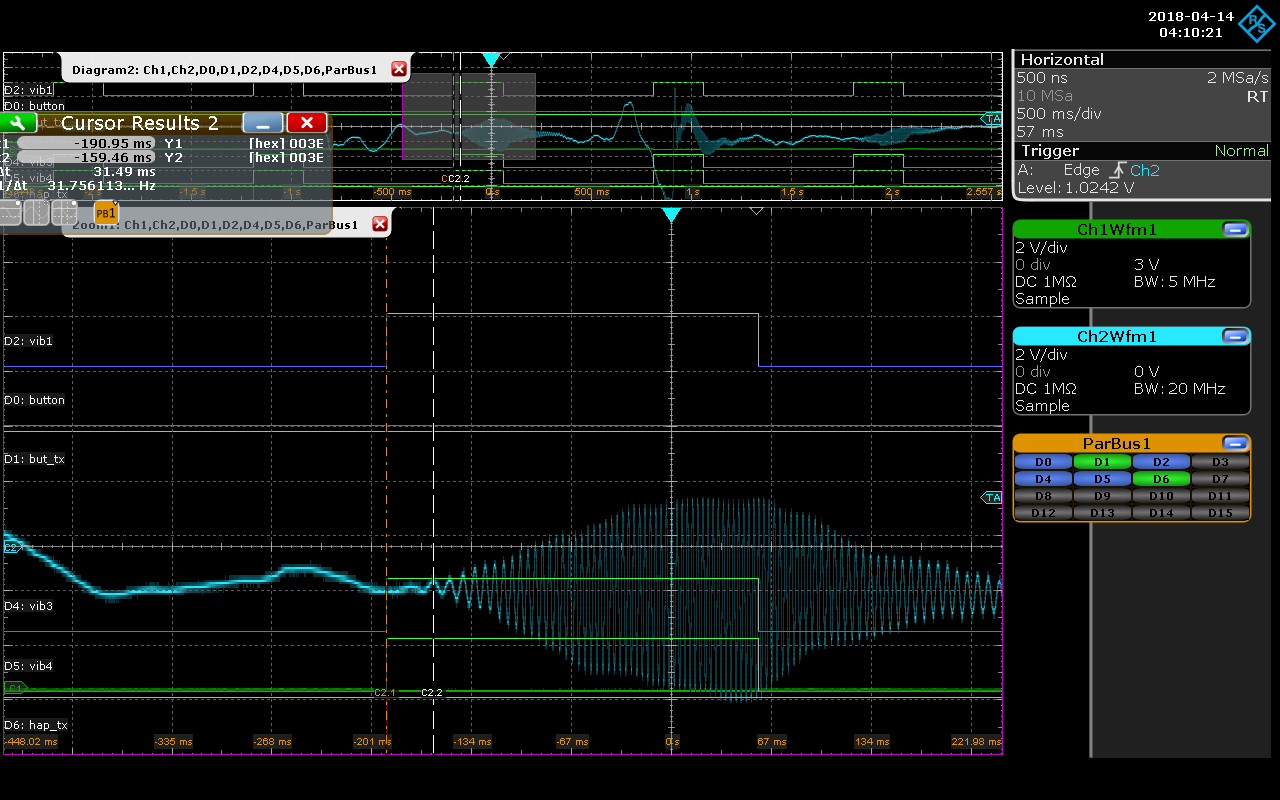
\includegraphics[width=\textwidth,height=\textheight,keepaspectratio]
    {motorramp2}
    \caption{$50ms$ motor ramp up time to perceptibility}
    \label{fig:MotorRampUp2}
\end{figure}

\subsection{Software}
The code was written in the Arduino IDE which utilizes C++. Outside of the tap tempo hardware push button, the main control flow was through serial communication over FTDI. The device communicated at 115200 baud and a small method was written to read the serial buffer and parse the incoming bytes into integers. The first input was a setter to store the current operation mode with 1 being the Discrete (Instantaneous) Mode and 2 Continuous. Afterwards, any other number (thresholded from 20 to 220) would be stored as the bpm. The period was calculated using formula \ref{eq:period}

The main control flow was two state machines which were delay independent. Depending on mode selection it would send digitalWrite commands to each motor within the set time period.
Though the analogWrite functionality built into the Arduino IDE could PWM the signal and potentially control the motor just below its turn on state, the transistors would not allow this due to their rapid speed and turn on voltage and the motors would be always vibrating. This was a design decision informed by the previous single vibrotactile prototype implementation.

The first state started a millisecond precision timer. In discrete mode the second state wrote all digitalIO pins HIGH for a quarter of the period as shown in Fig \ref{fig:state1}. A half on/off implementation was considered but determined to be not as efficient in communicating rapid pulses since the ramp down time overlapped with the next on period. During this state a flag was printed over serial to be read in later indicating when the test software could timestamp the onset.

\begin{lstlisting}[language=C]
    void go(){
        if(discrete==true){
            switch (newState){
              case READY:
                if(start){
                  average = avg;
                  startTime=millis();
                  newState++;
                }
                break;
              case ON: 
                digitalWrite(vibPins[0],HIGH);
                digitalWrite(vibPins[1],HIGH);
                digitalWrite(vibPins[2],HIGH);
                digitalWrite(vibPins[3],HIGH);
                if((millis()-startTime) >= ((average * 1)/4)){
                  newState++;
                  Serial.println("onset");
                }
                break;
              case OFF:
                digitalWrite(vibPins[0],LOW);
                digitalWrite(vibPins[1],LOW);
                digitalWrite(vibPins[2],LOW);
                digitalWrite(vibPins[3],LOW);
                if(millis()-startTime >= average){
                  newState=0;
                }
                break;
              default:
                break;
            }
        }
\end{lstlisting}
% \caption{Discrete/Instantaneous state machine}

The state machine in continuous mode functioned similarly but was divided into 4 ramp-up states and 4 ramp-down states as shown in Fig \ref{fig:state2}. Each state held its vibrotactile high for 1/9 of the overall period or IOI but lingered on the fourth vibrotactile slightly longer \textit{(2/9th's * IOI)} to convey the pinnacle of the beat. This state also sent the onset trigger.

% \caption{Continous state machine}
\begin{lstlisting}[language=C]
    if(discrete==false){
        switch (state) {
          case START:
            if(start){
              average = avg;
              startTime=millis(); 
              state++;
            }
            break;
          case RAMPUP_STEP_1:
            digitalWrite(vibPins[0],HIGH);
            if((millis()-startTime) >= ((average * 1)/9)){
              state++;
            }
            break;
          case RAMPUP_STEP_2:
            digitalWrite(vibPins[0],LOW);
            digitalWrite(vibPins[1],HIGH);
            if((millis()-startTime) >= ((average * 2)/9)){
              state++;
            }
            break;
          case RAMPUP_STEP_3:
            digitalWrite(vibPins[1],LOW);
            digitalWrite(vibPins[2],HIGH);
            if((millis()-startTime) >= ((average * 3)/9)){
              state++;
            }
            break;
          case RAMPUP_STEP_4:
            digitalWrite(vibPins[2],LOW);
            digitalWrite(vibPins[3],HIGH);
            if((millis()-startTime) >= ((average * 5)/9)){
              state++;
              Serial.println("onset");
            }
            break;
          case RAMPDOWN_STEP_5:
            digitalWrite(vibPins[3],LOW);
            digitalWrite(vibPins[2],HIGH);
            if((millis()-startTime) >= ((average * 6)/9)){
              state++;
            }
            break;
          case RAMPDOWN_STEP_6:
            digitalWrite(vibPins[2],LOW);
            digitalWrite(vibPins[1],HIGH);
            if((millis()-startTime) >= ((average * 7)/9)){
              state++;
            }
            break;
          case RAMPDOWN_STEP_7:
            digitalWrite(vibPins[1],LOW);
             digitalWrite(vibPins[0],HIGH);
            if((millis()-startTime) >= ((average * 8)/9)){
              state++;
            }
            break;
           case END:
              digitalWrite(vibPins[0],LOW);
             if((millis()-startTime) >= average){
               state=0; 
             }
            break;
          default:
            break;
        }
      }
\end{lstlisting}